\documentclass{article}
\usepackage[utf8]{inputenc}
\usepackage[english, russian]{babel}
\usepackage{hyperref}
\usepackage{graphicx}
\usepackage{minted}

\begin{document}

\title{Запросы \texttt{SPARQL}}
\author{Кравченко Дима, СПб ВШЭ, 5й курс}

\maketitle

Оригинальный гист (там лучше форматировано, так что лучше смотреть его):
\url{https://gist.github.com/equivalence1/79be410acd7bc4ad61ca4a1ced0592ea#file-task-md}

В этом pdf'e фиговая копия gist'a.

\section*{Task 1}

\subsection*{Description}
Призеры зимних Олимпийских игр 2018 в дисциплине "скелетон".
\subsection*{Solution}

Этот запрос я делал к базе dbpedia. На мой взгляд, идиологически правильным должен быть вот такой запрос:

\begin{minted}{sparql}
PREFIX owl: <http://www.w3.org/2002/07/owl#>
PREFIX xsd: <http://www.w3.org/2001/XMLSchema#>
PREFIX rdfs: <http://www.w3.org/2000/01/rdf-schema#>
PREFIX rdf: <http://www.w3.org/1999/02/22-rdf-syntax-ns#>
PREFIX foaf: <http://xmlns.com/foaf/0.1/>
PREFIX dc: <http://purl.org/dc/elements/1.1/>
PREFIX : <http://dbpedia.org/resource/>
PREFIX dbpedia2: <http://dbpedia.org/property/>
PREFIX dbpedia: <http://dbpedia.org/>
PREFIX skos: <http://www.w3.org/2004/02/skos/core#>

PREFIX dco: <http://dbpedia.org/ontology/>
PREFIX dct: <http://purl.org/dc/terms/>
PREFIX dbr: <http://dbpedia.org/resource/>
PREFIX dbc: <http://dbpedia.org/resource/Category:>

SELECT ?sportsman
FROM <http://dbpedia.org/>
WHERE {
     { dbr:Skeleton_at_the_2018_Winter_Olympics dbo:goldMedalist ?sportsman . }
     UNION
     { dbr:Skeleton_at_the_2018_Winter_Olympics dbo:silverMedalist ?sportsman . }
     UNION
     { dbr:Skeleton_at_the_2018_Winter_Olympics dbo:bronzeMedalist ?sportsman . }
}
\end{minted}

\subsection*{Notes}

К сожалению, это работает только для олимпийских игр до 2006 года включительно (т.е. если везде заменить 2018 на 2006, то все корректно
отработает для 2006 года). Это связанно с тем, что в dbpedia не проставленны медалисты по скелетону после 2006 года.
А если какие-то и заданы, то они, почему то, отдельны заданы по мужчинам, отдельно по женщинам (см \url{http://dbpedia.org/page/Skeleton\_at\_the\_2014\_Winter\_Olympics\_\%E2\%80\%93\_Women's} and \url{http://dbpedia.org/page/Skeleton\_at\_the\_2014\_Winter\_Olympics\_\%E2\%80\%93\_Men's}) 

В любом случае, вообще никакой информации по призерам зимних олимпийских игр 2018 на dbpedia я не нашел и учитывая, что
искал довольно много, практически уверен, что ее нет.

Далее, этот запрос можно немного постараться улучшить, если искать отдельно по женщинам и мужчинам (например, вот entity для
женщин 2014 года, где указаны призеры: \url{http://dbpedia.org/page/Skeleton\_at\_the\_2014\_Winter\_Olympics\_\%E2\%80\%93\_Women's}).

Насколько я понимаю, если сделать UNION из 6-ти таких штук (3 для мужчин и 3 для женщин), то можно достать результаты вплоть
до 2014 года. К сожалению, самого запроса у меня написать не получилось. Из-за наличия символов `–` и `'` в ссылке,
у меня вообще не получается ее использовать в SPARQL endpoint'e. Сервер отказывается это парсить. Я даже скачал сами
тройки dbpedia и вставлял ссылки вида \\ \texttt{<http://dbpedia.org/resource/Skeleton\_at\_the\_2014\_Winter\_Olympics\_\\u2013\_Women\\u0027s>}, но это не дает никаких результатов (я попробовал еще 
несколько вариантов преобразования линки, но SPARQL либо тупо не парсит, либо ничего не находит, хотя должен).

Можно его сделать совсем работающим до 2014 года включительно, если предположить, что все скелетонисты участвовали
исключительно в скелетоне. Тогда можно сформировать такой запрос:

\begin{minted}{sparql}
PREFIX owl: <http://www.w3.org/2002/07/owl#>
PREFIX xsd: <http://www.w3.org/2001/XMLSchema#>
PREFIX rdfs: <http://www.w3.org/2000/01/rdf-schema#>
PREFIX rdf: <http://www.w3.org/1999/02/22-rdf-syntax-ns#>
PREFIX foaf: <http://xmlns.com/foaf/0.1/>
PREFIX dc: <http://purl.org/dc/elements/1.1/>
PREFIX : <http://dbpedia.org/resource/>
PREFIX dbpedia2: <http://dbpedia.org/property/>
PREFIX dbpedia: <http://dbpedia.org/>
PREFIX skos: <http://www.w3.org/2004/02/skos/core#>

PREFIX dco: <http://dbpedia.org/ontology/>
PREFIX dct: <http://purl.org/dc/terms/>
PREFIX dbr: <http://dbpedia.org/resource/>
PREFIX dbc: <http://dbpedia.org/resource/Category:>

SELECT ?sportsman
FROM <http://dbpedia.org/>
WHERE {
     { ?sportsman dct:subject dbc:Medalists_at_the_2014_Winter_Olympics ,
                              dbc:Skeleton_racers_at_the_2014_Winter_Olympics . }
}
\end{minted}

Замечу, что он написан для 2014 года. За 2018 все равно нет записей. Так же еще раз замечу, что этот запрос верен
только в том случае, если никакой скелетонист не участвовал в чем-то, кроме скелетона, и не взял там медаль (на деле таких случаев нет, так что запрос отрабатывает корректно для всех годов).

\subsection*{Results}

Приведены для нижнего запроса (2014 год, за 2018 не интересно, там пусто).

\noindent\makebox[\textwidth]{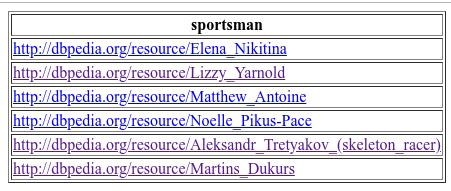
\includegraphics[width=\textwidth]{task-1.png}}
 
\section*{Task 2}

\subsection*{Description}

Суда с портом приписки Сочи.

\subsection*{Solution}

Это запрос к endpoint'у wikidata

\begin{minted}{sparql}
SELECT DISTINCT ?ship
WHERE {
  ?ship (wdt:P31/wdt:P279*) wd:Q11446 .
  ?ship wdt:P532 wd:Q4430373 .
}
\end{minted}

\subsection*{Notes}
Кажется, он ничего не возвращает. Причин может быть две. Первая -- в wikidata действительно нет записей о судах с
портом приписки Сочи. Второй -- wikidata явно ограничивает длину обхода графа. Например, запрос вида \texttt{?ship (wdt:P31/wdt:P279*) wd:Q11446 .} (т.е. все те entity, которые прямо или косвенно являются instance of ship). Не выдает яхту A (\url{https://www.wikidata.org/wiki/Q300311}). Но вот запрос \texttt{?ship (wdt:P31/wdt:P279*) wd:Q170173 .} (т.е. все те entity, которые прям или косвенно являются instance of yacht). При этом 1) яхта А не является прямым instance'ом класса yacht 2) yacht это subclass of ship. Поэтому видно, что при том, что я задал произвольную глубину наследования (\texttt{wdt:P279*}),
wikidata ушел только на глубину 2 (A instance of motor yacht, motor yacht subclass of yacht), а на глубину 3 (yacht subclass of ship) уже не пошел.
\subsection*{Results}

\noindent\makebox[\textwidth]{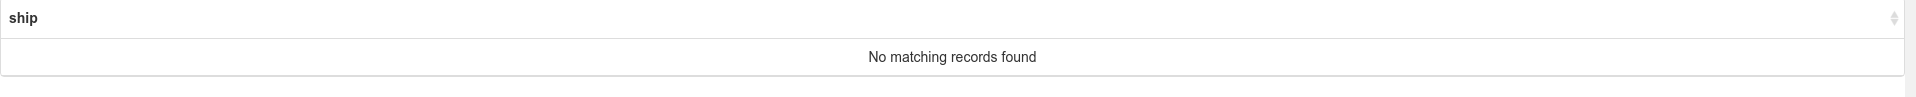
\includegraphics[width=\textwidth]{task-2.png}}

\section*{Task 3}

\subsection*{Description}
Общее количество произведений Агаты Кристи; годы издания первой и последней книги Агаты Кристи.
\subsection*{Solution}

Это запрос к endpoint'у YAGO.

\begin{minted}{sparql}
PREFIX owl: <http://www.w3.org/2002/07/owl#>
PREFIX xsd: <http://www.w3.org/2001/XMLSchema#>
PREFIX rdfs: <http://www.w3.org/2000/01/rdf-schema#>
PREFIX rdf: <http://www.w3.org/1999/02/22-rdf-syntax-ns#>
PREFIX foaf: <http://xmlns.com/foaf/0.1/>
PREFIX dc: <http://purl.org/dc/elements/1.1/>
PREFIX : <http://yago-knowledge.org/resource/>
PREFIX skos: <http://www.w3.org/2004/02/skos/core#>

PREFIX dct: <http://purl.org/dc/terms/>

SELECT (COUNT(DISTINCT ?work) AS ?work_count) (MIN(?year) AS ?min_year) (MAX(?year) AS ?max_year)
WHERE {
    :Agatha_Christie :created ?work .
    OPTIONAL { ?work :wasCreatedOnDate ?date . }
    BIND(REPLACE(str(?date), "(\\d{4}).*", "$1") AS ?year)
    ?work skos:prefLabel ?skosLabel .
    FILTER (!REGEX(?skosLabel, "film\\)", "i"))
}
\end{minted}
\subsection*{Notes}

Тут есть некоторые проблемы связанные с тем, что:

1. Не все произведения имеют проставленную дату. 

2. Некоторые фильмы, которые были сняты по произведниям Агаты Кристи считаются created by Agatha\_Christie. Более того,
единственный способ, который я нашел, чтобы разделить книги и фильмы -- это пропарсить их \texttt{skos:prefLabel} (к счастью,
они все его имеют, и для всех фильмов строка кончается на "film)"). Можно было бы лучше (идеологически лучше) понять, фильм это или книга, если посмотреть на проперти \texttt{sameAs}, который ведет на entity из dbpedia, а в ней уже нормально
указано, книга это или фильм. Но если так делать, то я не очень понимаю, в чем вообще смысл использования endpoint'a YAGO? В любом случае, хоть это и криво, но способ с парсингом label'a работает.
\subsection*{Results}

\noindent\makebox[\textwidth]{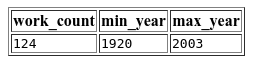
\includegraphics[width=\textwidth]{task-3.png}}

\section*{Task 4}

\subsection*{Description}

Внуки и внучки королевы Англии Елизаветы II.
\subsection*{Solution}

Этот запрос к dbpedia:

\begin{minted}{sparql}
PREFIX owl: <http://www.w3.org/2002/07/owl#>
PREFIX xsd: <http://www.w3.org/2001/XMLSchema#>
PREFIX rdfs: <http://www.w3.org/2000/01/rdf-schema#>
PREFIX rdf: <http://www.w3.org/1999/02/22-rdf-syntax-ns#>
PREFIX foaf: <http://xmlns.com/foaf/0.1/>
PREFIX dc: <http://purl.org/dc/elements/1.1/>
PREFIX : <http://dbpedia.org/resource/>
PREFIX dbpedia2: <http://dbpedia.org/property/>
PREFIX dbpedia: <http://dbpedia.org/>
PREFIX skos: <http://www.w3.org/2004/02/skos/core#>

PREFIX dco: <http://dbpedia.org/ontology/>
PREFIX dct: <http://purl.org/dc/terms/>
PREFIX dbr: <http://dbpedia.org/resource/>
PREFIX dbc: <http://dbpedia.org/resource/Category:>

SELECT ?h
FROM <http://dbpedia.org/>
WHERE {
     { ?child dbo:parent dbr:Elizabeth_II . }
     { ?h dbo:parent ?child . }
}
\end{minted}
\subsection*{Notes}
Вроде находит всех, судя по той информации, что я нашел на просторах интернета.
\subsection*{Results}

\noindent\makebox[\textwidth]{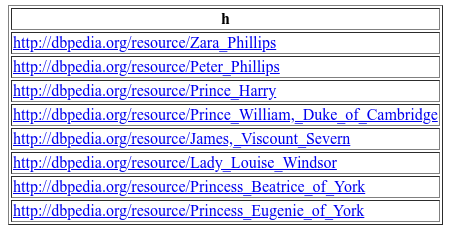
\includegraphics[width=\textwidth]{task-4.png}}

\section*{Task 5}

\subsection*{Description}
Романы Владимира Набокова, которые в оригинале были написаны 1) по-русски, 2) по-английски. 
\subsection*{Solution}
Это запрос к endpoint'у Wikidata

\begin{minted}{sparql}
SELECT ?orig_lang_code (COUNT(DISTINCT ?work) AS ?num_works)
WHERE {
    ?work wdt:P50 wd:Q36591 .
    ?work wdt:P31 wd:Q571 .
    ?work (wdt:P136/wdt:P279*) wd:Q8261 .
    ?work wdt:P407 ?orig_lang .
    ?orig_lang wdt:P219 ?orig_lang_code .
}
GROUP BY ?orig_lang_code
\end{minted}

Такой запрос одновременно выдаст результаты для всех языков, решая сразу пункты 1) и 2). Если хочется
выдавать результаты только для одного языка, например английского, то можно добавить \texttt{FILTER(?orig\_lang\_code = "eng")}. 
Итоговый запрос для английского языка будет выглядеть так:

\begin{minted}{sparql}
SELECT (COUNT(DISTINCT ?work) AS ?num_works)
WHERE {
    ?work wdt:P50 wd:Q36591 .
    ?work wdt:P31 wd:Q571 .
    ?work wdt:P136/wdt:P279* wd:Q8261 .
    ?work wdt:P407 ?orig_lang .
    ?orig_lang wdt:P219 ?orig_lang_code .
    FILTER (?orig_lang_code="eng") .
}
\end{minted}

Для русского: 

\begin{minted}{sparql}
SELECT (COUNT(DISTINCT ?work) AS ?num_works)
WHERE {
    ?work wdt:P50 wd:Q36591 .
    ?work wdt:P31 wd:Q571 .
    ?work wdt:P136/wdt:P279* wd:Q8261 .
    ?work wdt:P407 ?orig_lang .
    ?orig_lang wdt:P219 ?orig_lang_code .
    FILTER (?orig_lang_code="rus") .
}
\end{minted}
\subsection*{Notes}
У этих запросов есть небольшая проблема. Дело в том, что произведение может иметь несколько пропертей "language of work or name", указывающих на разные языки. Поэтому сумма этих 2х чисел будет больше, чем всего романов у Набокова.
Как минимум средствами wikidata с этим не побороться. Возможно, можно обратиться к какому-нибудь стороннему сервису
с помощью SERVICE, но я даже не знаю, к какому можно, чтобы там все нормально отработало.

\subsection*{Results}

Приведены для верхнего запроса, который считает сразу для всех языков.

\noindent\makebox[\textwidth]{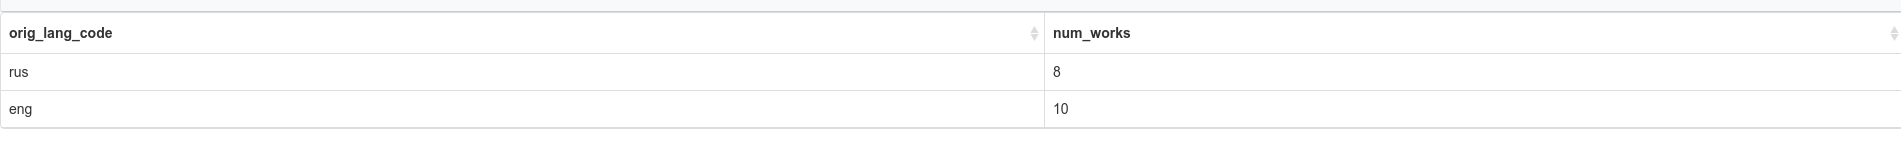
\includegraphics[width=\textwidth]{task-5.png}}

\section*{Task 6}

\subsection*{Description}

Дополните эксперимент своими запросами.

Я решил для каждого века нашей эры посчитать, сколько физиков теоретиков в нем было рождено.
\subsection*{Solution}
Это запрос к wikidata

\begin{minted}{sparql}
SELECT (xsd:integer(?cent) AS ?cent) (COUNT(DISTINCT ?human) AS ?phys_born)
WHERE {
  ?human wdt:P31 wd:Q5 .
  ?human (wdt:P106/wdt:P279*) wd:Q169470 .
  ?human wdt:P569 ?date_of_birth .
  FILTER (!REGEX(str(?date_of_birth), ".*BCE.*", "i"))
  BIND(REPLACE(str(?date_of_birth), "(\\d{4}).*", "$1") AS ?year)
  BIND(REPLACE(str(?year), "(\\d{2}).*", "$1") AS ?cent)
  FILTER (xsd:integer(?cent) > 0)  
}
GROUP BY ?cent
ORDER BY ?cent
\end{minted}
\subsection*{Notes}
Почему-то проверки на наличие "BCE" в строке не хватает. Он все равно возврщает записи до нашей эры. По этому приходится делать еще одну проверку на `xsd:integer(?cent) > 0`. Тогда все нормально работает.

\subsection*{Results}

\noindent\makebox[\textwidth]{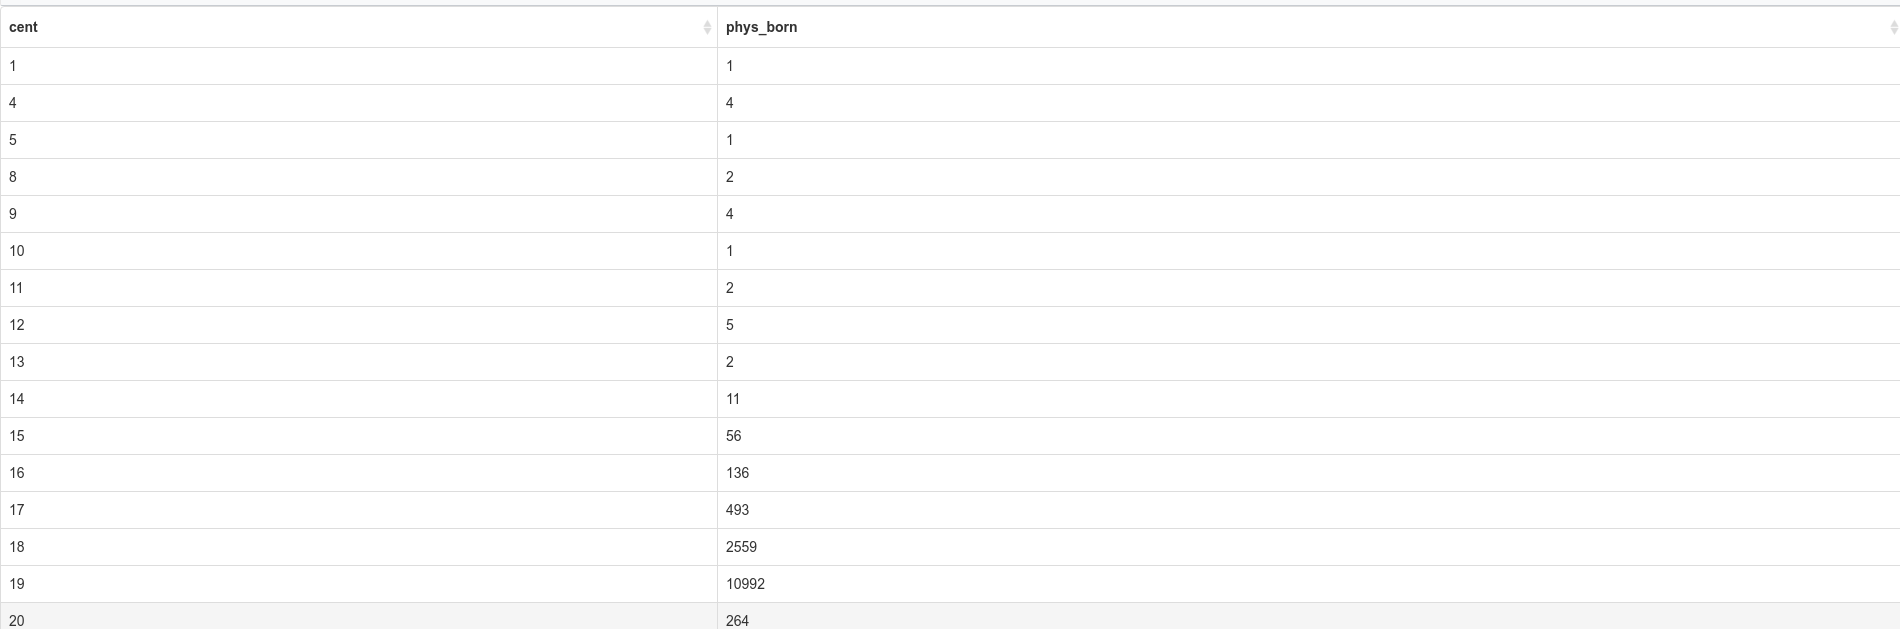
\includegraphics[width=\textwidth]{task-6.png}}

\end{document}